\subsection{Optimization Results}\label{sec:optimization_results}
In this section, we present and analyze the results of running the optimization experiment that we described in Section~\ref{subsec:optimization_experiment_design}.
As mentioned, our primary objective was to identify the optimal configurations for predicting the concentration of various oxides in our dataset.
We systematically evaluated a range of machine learning models, preprocessing techniques, and hyperparameter settings to determine the most effective combinations for each oxide.

The results of the experiment were ~$16.000$ trials worth of data on the configurations used, hyperparameters, as well as metrics.

Our data cleaning for this dataset primarily included filtering out failed runs, which was caused by configurations that did not work well together, as well as filtering out extreme error values.
We filter out any runs that had an \gls{rmsecv} above 50.
Approaches like \gls{svr} could occasionally yield this kind of outlier result in specific configurations.
We chose a threshold of 50 to include as many trials that were not clearly outliers.

Our experiment proceeded mostly without encountering any issues.
Some issues are to be expected given the scale of the experiment.
Unfortunately, we encountered an issue with a server we were using, resulting in some oxides and models having to be re-run.
We managed to recover and re-run most of these.
However, \gls{ngboost} for \ce{MgO} was only partially finished.
Given that each model of the ten models would undergo 200 trials, for each oxide, this resulted in 2000 runs per oxide.
The exception is \ce{MgO}, for which \gls{ngboost} ran 143 trials, making the total trials for \ce{MgO} 1943.
After the filtering process, we are left with a total of 15245 trials to analyze.

Since we stored the configurations as well as each hyperparameter value for the trials, we had \~100 variables to consider during our analysis.
Among these, the primary variables of interest are the metrics and overall configuration variables, namely \texttt{Model Type}, \texttt{Scaler Type}, \texttt{PCA Type}, and \texttt{Transformer Type}.

We used this data to identify the best configurations for each oxide, as measured by \gls{rmsecv}.
We began our analysis broadly by examining the usage of preprocessors across trials. Subsequently, we narrowed our focus and reviewed the top 100 trials for each oxide to identify the optimal model, scaler, and transformer for each oxide.
Finally, we examined the single best-performing configurations across oxides, showing one configuration per model for each oxide.

As described in Section~\ref{sec:optimization_framework}, our optimization system searches for the best configurations through multi-objective optimization.
The optimization process involves adjusting the configuration and hyperparameters of the machine learning model and preprocessing pipeline to minimize the objective.
As the sampler conducts initial exploration and subsequently seeks to identify the optimal configuration through exploitation, we expect that the values of variables frequently appearing in the results are most likely to be optimal.
Table \ref{tab:scalers_comparison}, \ref{tab:pca_comparison}, and \ref{tab:transformers_comparison} display these values for the various preprocessors.
The optimization results indicate that configurations with the highest total values across oxides are often the most frequently exploited, suggesting they are most likely to optimize performance.
\texttt{Norm3Scaler} was used in 5090 trials, and therefore appears to be the most effective scaler.
This outcome was expected, as the method was specifically designed for this type of \gls{libs} dataset, as discussed in Section~\ref{sec:norm3}.
For dimensionality reduction, we see that \texttt{None}, indicating no \gls{pca}, was used in 9419 trials, constituting approximately 59\% of all trials.
This suggests that either no dimensionality reduction is optimal, or a more suitable method should be identified.
Neither \gls{pca} nor \gls{kernel-pca} appear to be effective for this dataset.
\texttt{QuantileTransformer} was used in 5710 trials, indicating that it may be the most optimal transformer.
We observe that \texttt{PowerTransformer} was employed in 5277 trials, while no transformer was used in 4956 trials. Unlike other preprocessing method types, there does not appear to be a clear winner for the transformers.

\begin{table*}
    \centering
    \begin{tabular}{lccccccccc}
        \toprule
        \textbf{Oxide} & \texttt{MaxAbsScaler} & \texttt{MinMaxScaler} & \texttt{Norm3Scaler} & \texttt{RobustScaler} & \texttt{StandardScaler} \\
        \midrule
        \ce{Al2O3}               & 336  & 476  & 495  & 453  & 240 \\
        \ce{CaO}                 & 310  & 362  & 681  & 338  & 309 \\
        \ce{FeO_T}               & 498  & 287  & 561  & 339  & 315 \\
        \ce{K2O}                 & 258  & 320  & 622  & 430  & 370 \\
        \ce{MgO}                 & 239  & 340  & 646  & 413  & 305 \\
        \ce{Na2O}                & 316  & 327  & 748  & 320  & 289 \\
        \ce{SiO2}                & 221  & 421  & 830  & 309  & 219 \\
        \ce{TiO2}                & 280  & 322  & 507  & 565  & 326 \\
        Total across oxides      & 2458 & 2855 & 5090 & 3167 & 2373 \\
        \bottomrule
    \end{tabular}
    \caption{Comparison of different scalers across the eight major oxides.}
    \label{tab:scalers_comparison}
\end{table*}


\begin{table*}
    \centering
    \begin{tabular}{lccccccccc}
        \toprule
        \textbf{Oxide} & \texttt{None} & \texttt{KernelPCA} & \texttt{PCA} \\
        \midrule
        \ce{Al2O3}               & 1243  & 389  & 368 \\
        \ce{CaO}                 & 1246  & 374  & 380 \\
        \ce{FeO_T}               & 1217  & 382  & 401 \\
        \ce{K2O}                 & 1250  & 373  & 377 \\
        \ce{MgO}                 & 1037  & 543  & 363 \\
        \ce{Na2O}                & 1167  & 382  & 451 \\
        \ce{SiO2}                & 1096  & 457  & 447 \\
        \ce{TiO2}                & 1163  & 468  & 369 \\
        Total across oxides      & 9419  & 3368 & 3156 \\
        \bottomrule
    \end{tabular}
    \caption{Comparison of different PCA types across the eight major oxides.}
    \label{tab:pca_comparison}
\end{table*}


\begin{table*}
    \centering
    \begin{tabular}{lccccccccc}
        \toprule
        \textbf{Oxide} & \texttt{None} & \texttt{PowerTransformer} & \texttt{QuantileTransformer} \\
        \midrule
        \ce{Al2O3}               & 442  & 649  & 909 \\
        \ce{CaO}                 & 673  & 595  & 732 \\
        \ce{FeO_T}               & 633  & 644  & 723 \\
        \ce{K2O}                 & 504  & 822  & 674 \\
        \ce{MgO}                 & 725  & 701  & 517 \\
        \ce{Na2O}                & 441  & 583  & 976 \\
        \ce{SiO2}                & 760  & 566  & 674 \\
        \ce{TiO2}                & 778  & 717  & 505 \\
        Total across oxides      & 4956 & 5277 & 5710 \\
        \bottomrule
    \end{tabular}
    \caption{Comparison of different transformers across the eight major oxides.}
    \label{tab:transformers_comparison}
\end{table*}

We chose to examine the top 100 trials for each configuration to provide a clearer understanding of the performance variance among the best configurations.
Given the wide range of configurations and their varying sensitivity to tuning, data distributions, and other factors, examining all trials would result in misleading descriptive statistics.
By focusing on the top 100 trials, we can more accurately identify which configurations perform well.
While a quantitative analysis of the top 10\% of trials based on metrics like \gls{rmsecv}, \gls{rmsep}, and other factors was feasible, selecting the top 100 trials for each oxide made it easier to see how many trials were present for each oxide.
This approach helps us avoid the 'best of the worst' scenario and ensures that we are analyzing a representative set of good configurations.
We present the results in Figure~\ref{fig:top100_models}, \ref{fig:top100_scalers}, \ref{fig:top100_transformers}, and \ref{fig:top100_pca}.
These figures and their corresponding subplots illustrate the performance of various configuration elements (models, scalers, transformers, PCA techniques) for each oxide, based on their \gls{rmsecv}.
Any elements that do not appear in a subplot were not used in the top 100 trials for the given oxide.
It is important to note that the variance in performance is influenced by multiple factors, not solely by the variable depicted in each plot.
Factors such as the interaction between different preprocessing techniques, specific hyperparameter settings, and the inherent variability in the data all contribute to the observed performance.
Therefore, while the plots offer valuable insights into the effectiveness of individual configuration elements, the overall performance is a result of complex interactions within the entire machine learning pipeline.
Therefore, we prioritize the analysis of the top-performing trials and examine a larger sample of these to draw generalizable conclusions about the optimal configurations for each oxide.

From Figure~\ref{fig:top100_models}, it is evident that \gls{svr}, gradient boosting methods, and \gls{pls} demonstrate the best performance.
Figure~\ref{fig:top100_pca} confirms our earlier hypothesis that not using any \gls{pca} or \gls{kernel-pca} yields the lowest \gls{rmsecv} values.
However, we do observe that either \gls{pca} or \gls{kernel-pca} appear in four of the plots, with \gls{kernel-pca} being the most frequently used among them.
This indicates that they are indeed used in some of the top-performing configurations.
Interestingly, Figure~\ref{fig:top100_scalers} shows that, although \texttt{Norm3Scaler} is the most frequently used and best-performing scaler, this is not always the case.
Min-max scaling appears to yield better results for \ce{SiO2} and \ce{CaO}, while robust scaling seems more effective for \ce{MgO}.
For \ce{Al2O3}, Norm 3 scaling exhibits the lowest \gls{rmsecv} values but a higher mean \gls{rmsecv} value compared to the other scalers.
Finally, Figure~\ref{fig:top100_transformers} reveals another nuanced finding.
Power transformations appear to most frequently yield the best results across oxides, while quantile transformation or no transformation show the lowest \gls{rmsecv} values for the remaining oxides.

These results further reinforce our hypothesis that a tailored configuration is necessary for each oxide, and there is no single configuration that performs well across all oxides.

\begin{figure*}
    \centering
    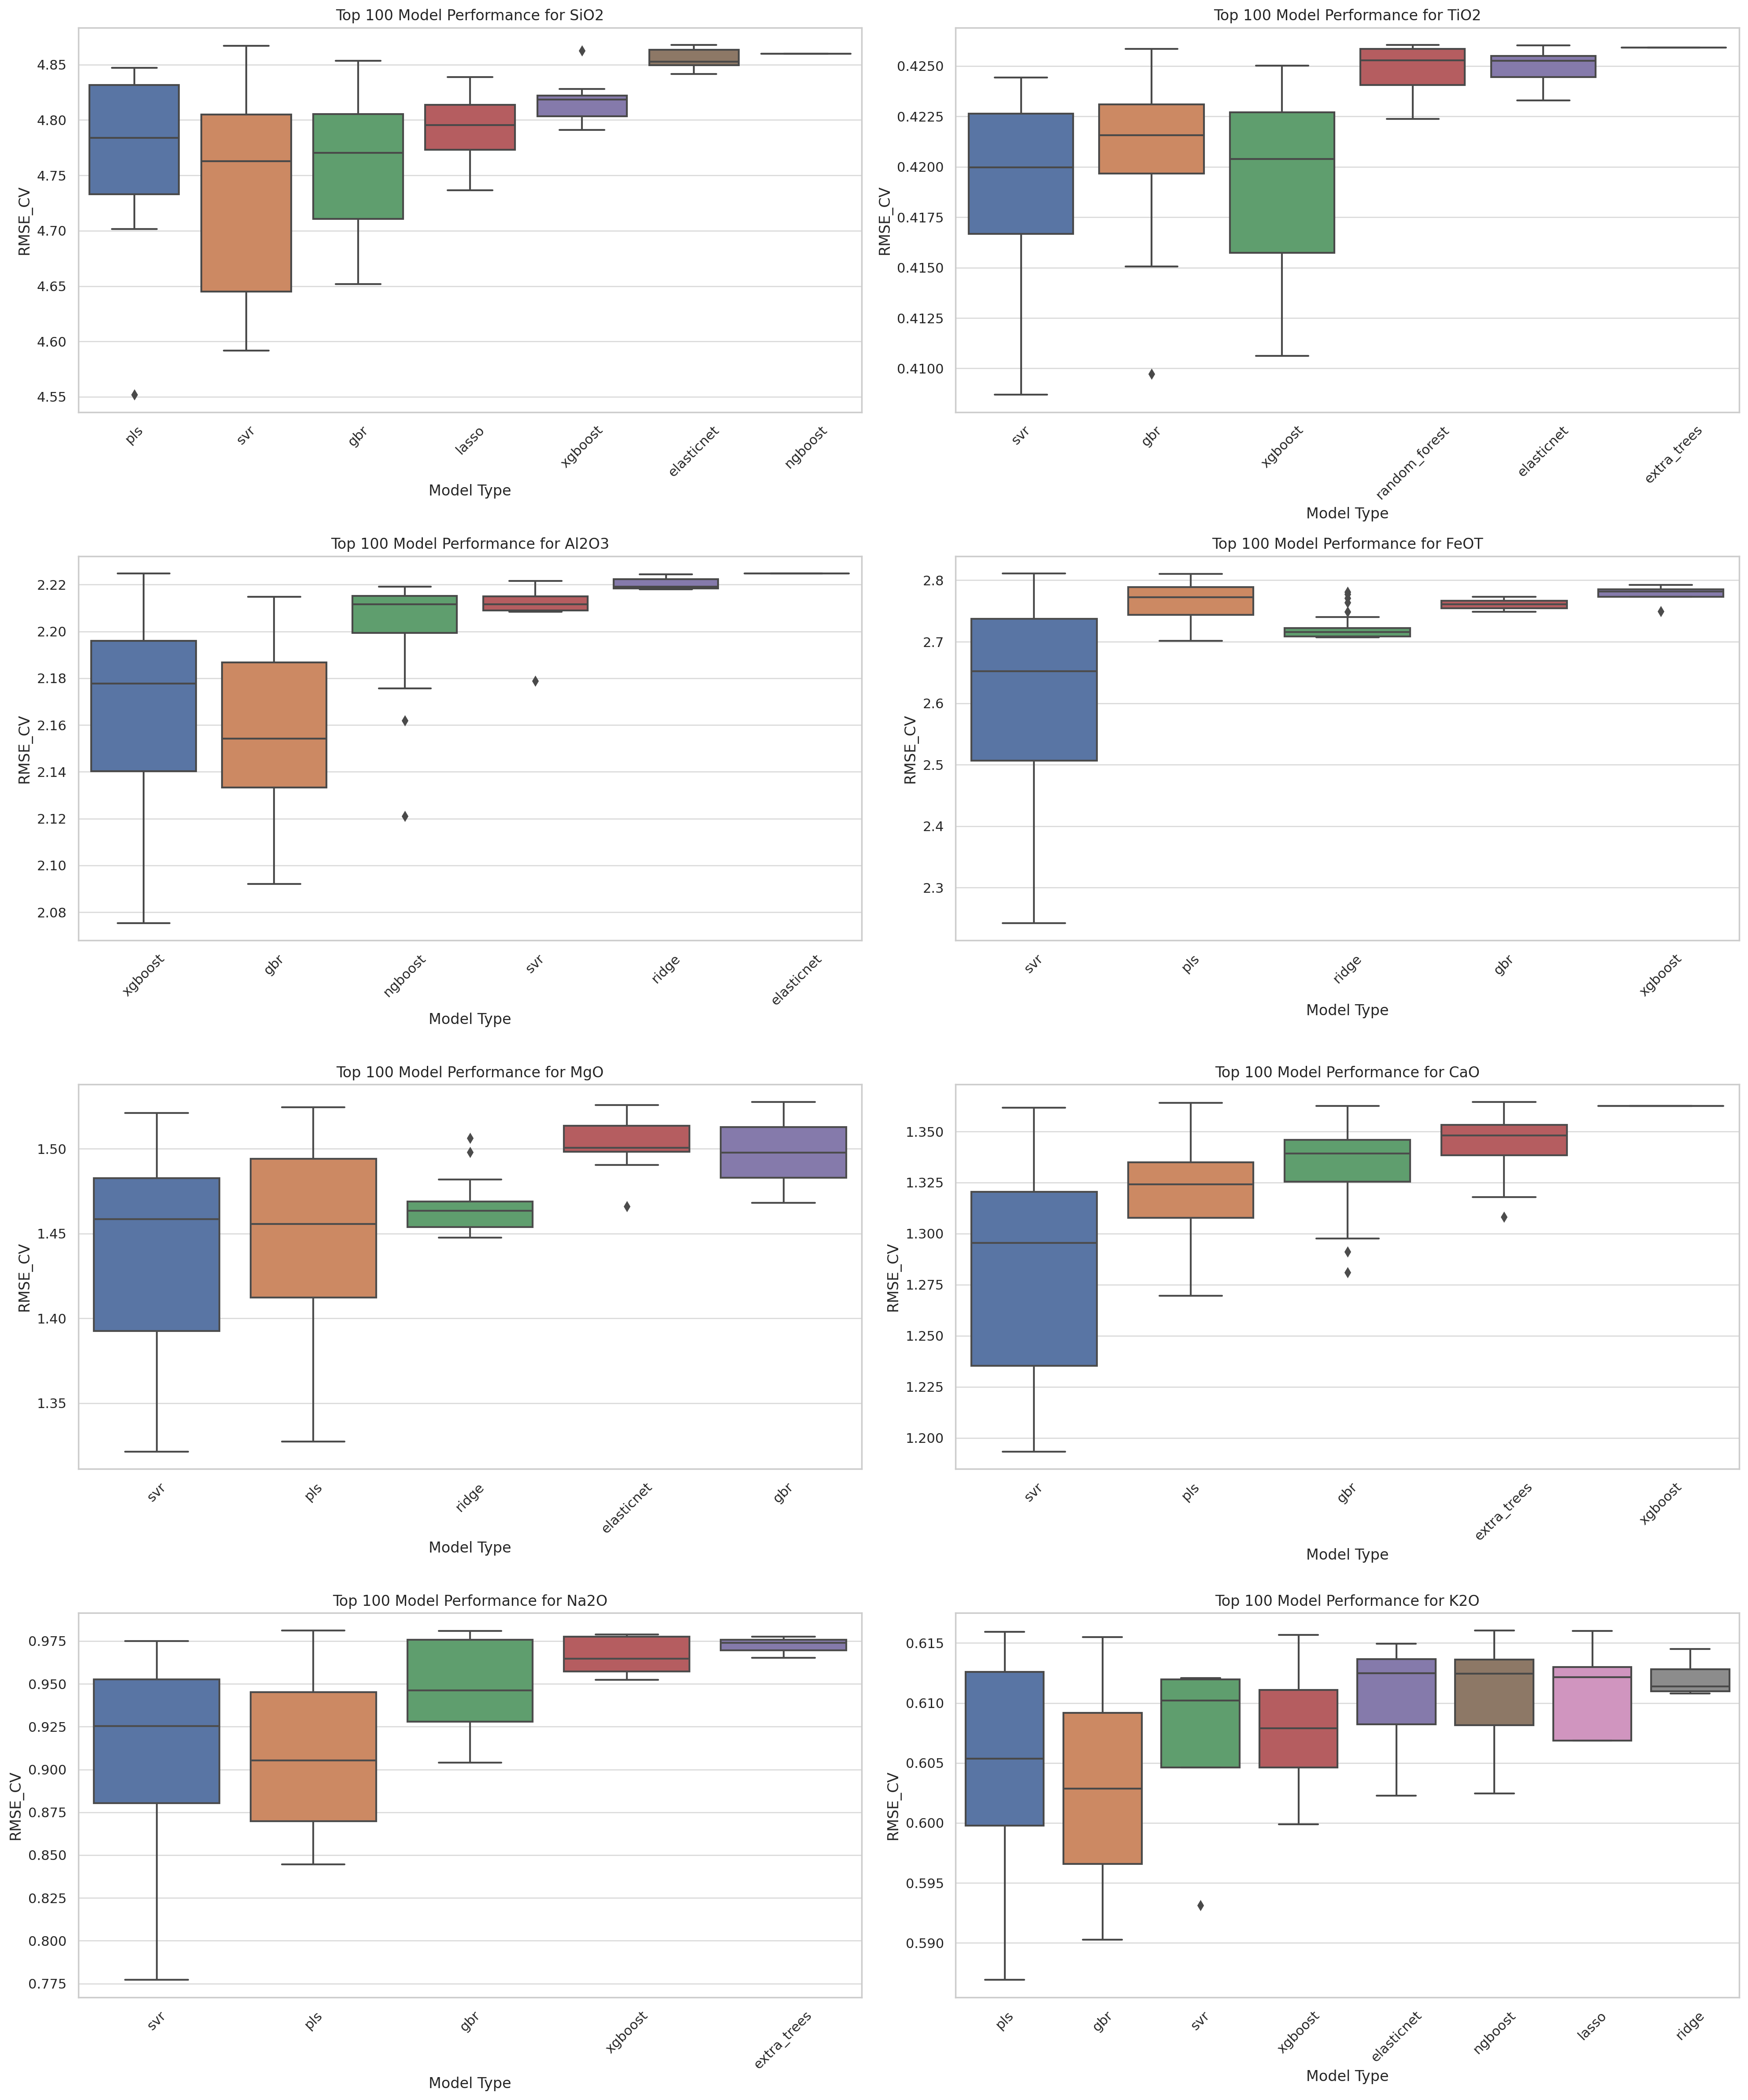
\includegraphics[width=\textwidth]{images/top100/models.png}
    \caption{Top 100 model performance across oxides. The subplots show the distribution of \gls{rmsecv} values for the top 100 trials for each model type across the eight different oxides. This helps identify the most effective models for each oxide within the top-performing trials.}
    \label{fig:top100_models}
\end{figure*}

\begin{figure*}
    \centering
    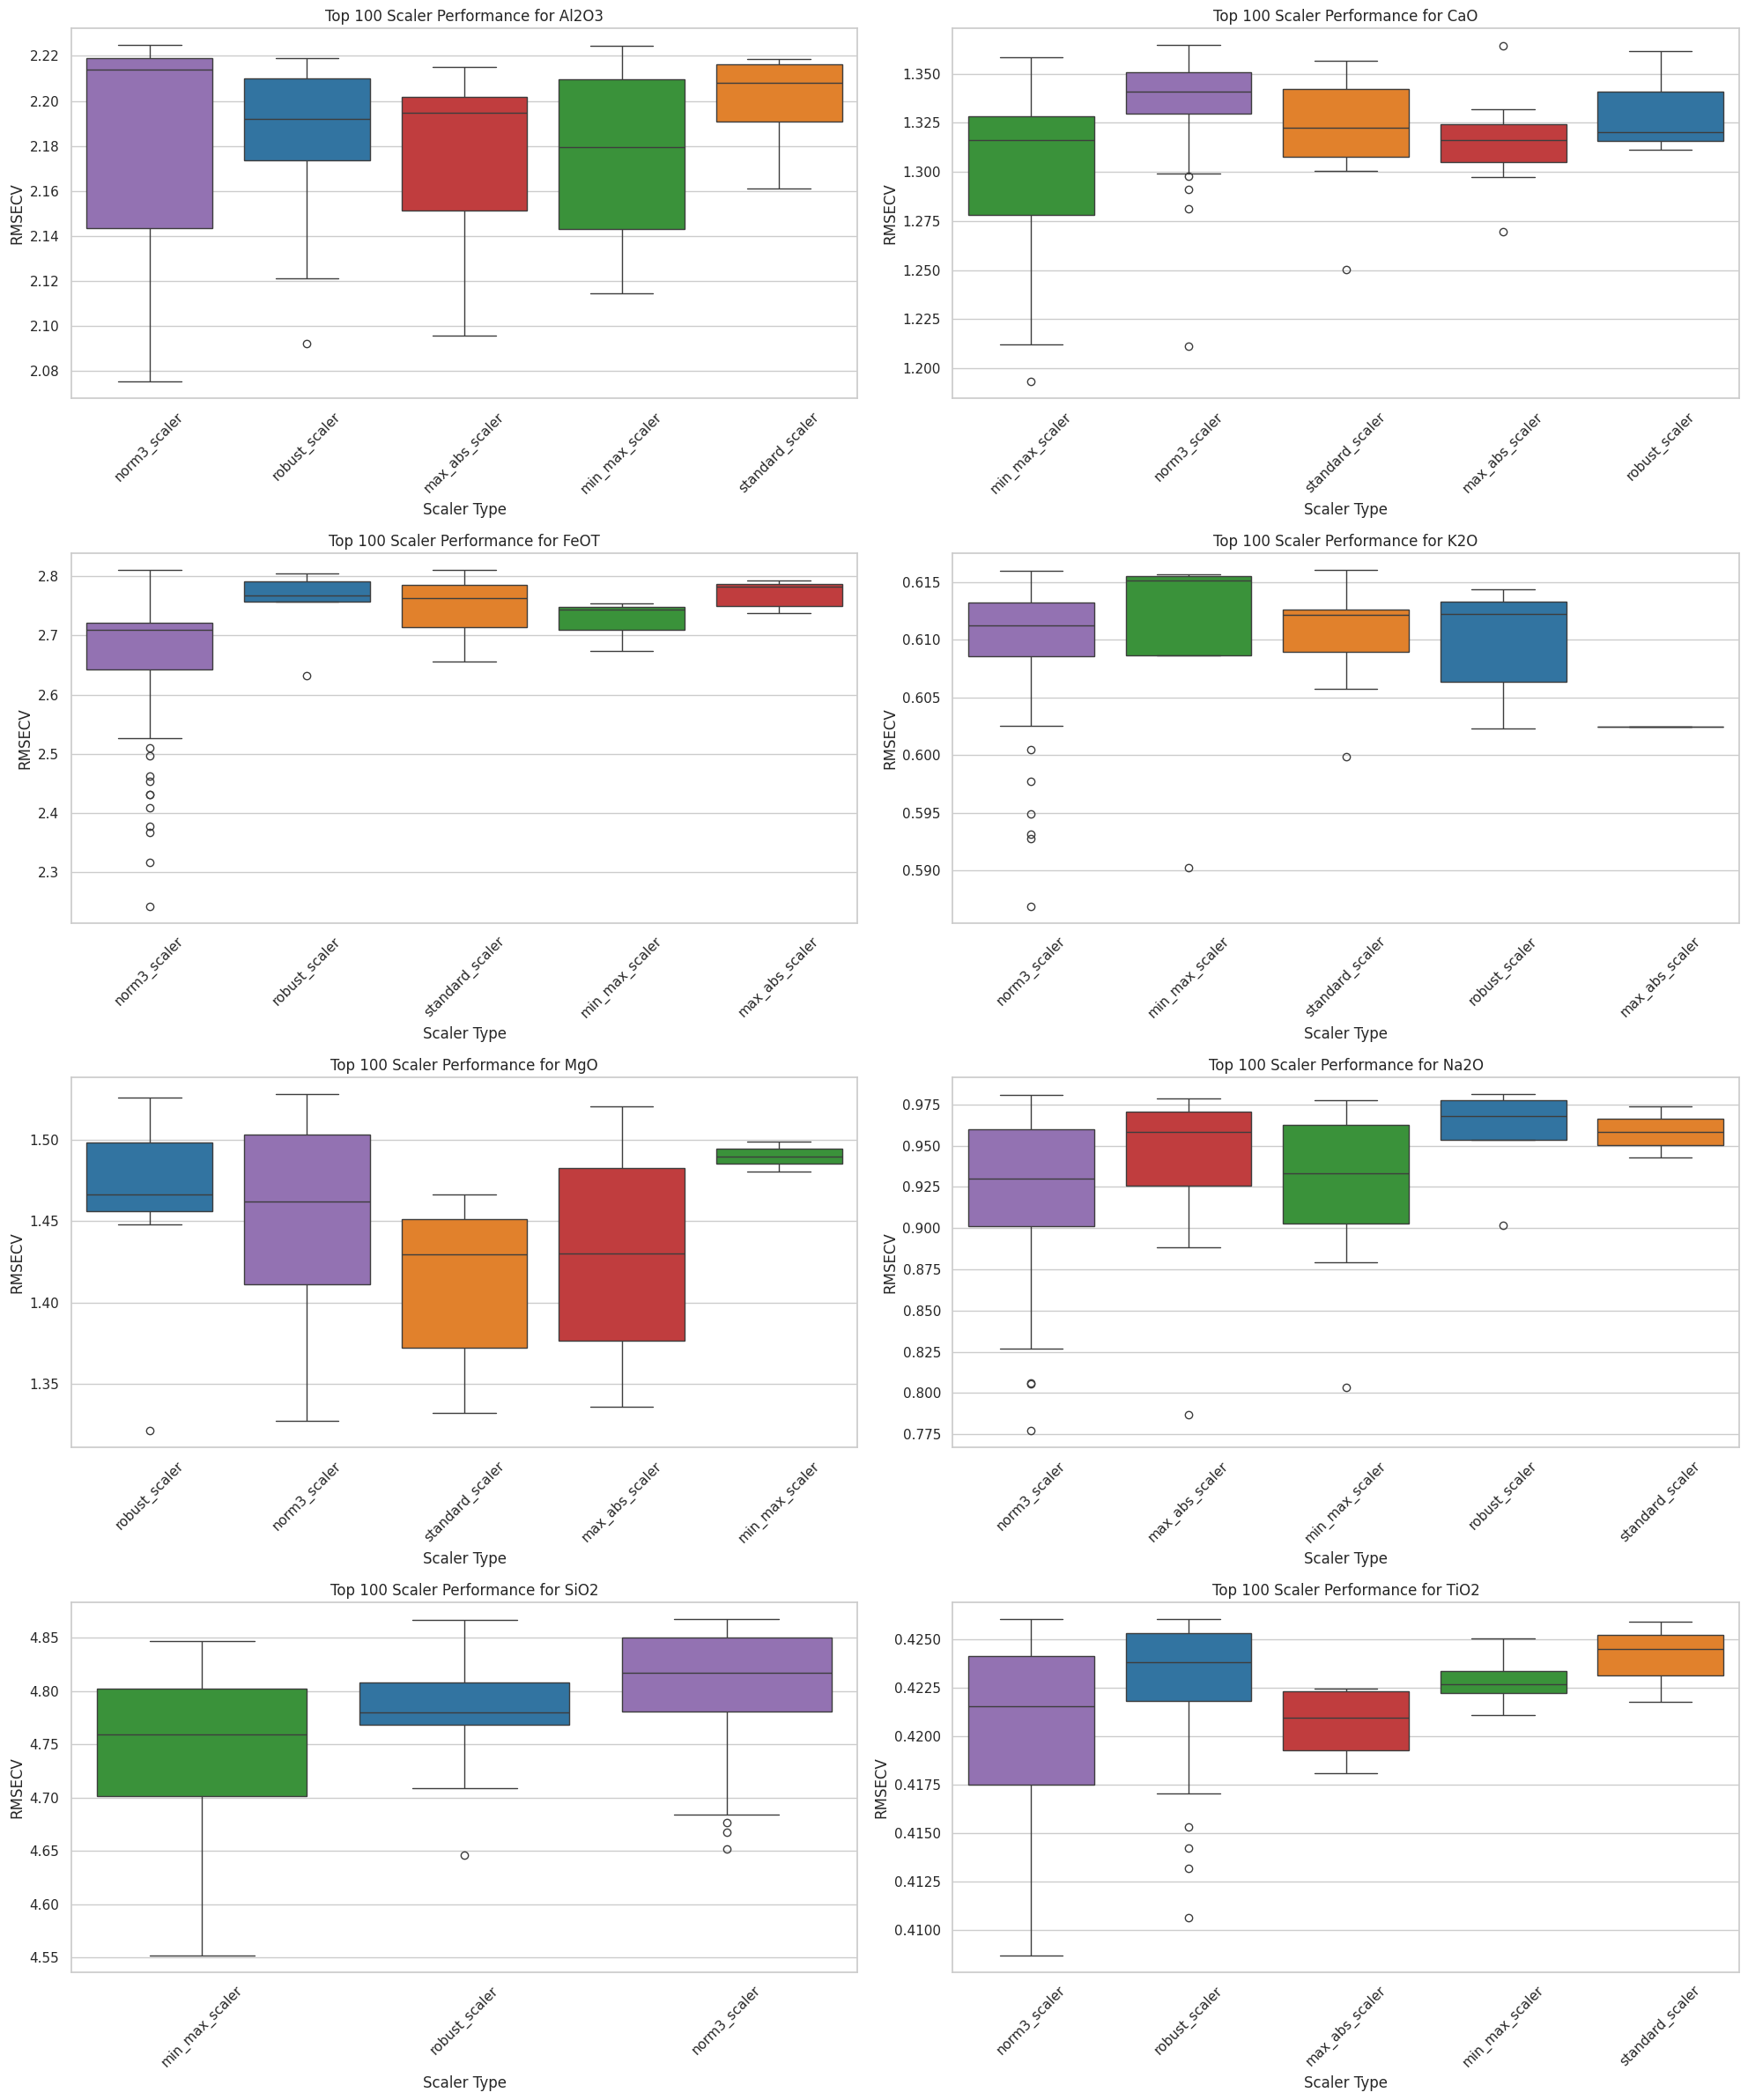
\includegraphics[width=\textwidth]{images/top100/scalers.png}
    \caption{Top 100 scaler performance across oxides. The subplots illustrate the distribution of \gls{rmsecv} values for the top 100 trials for each scaler type across the different oxides. This helps pinpoint which scalers perform best within the top-performing trials.}
    \label{fig:top100_scalers}
\end{figure*}

\begin{figure*}
    \centering
    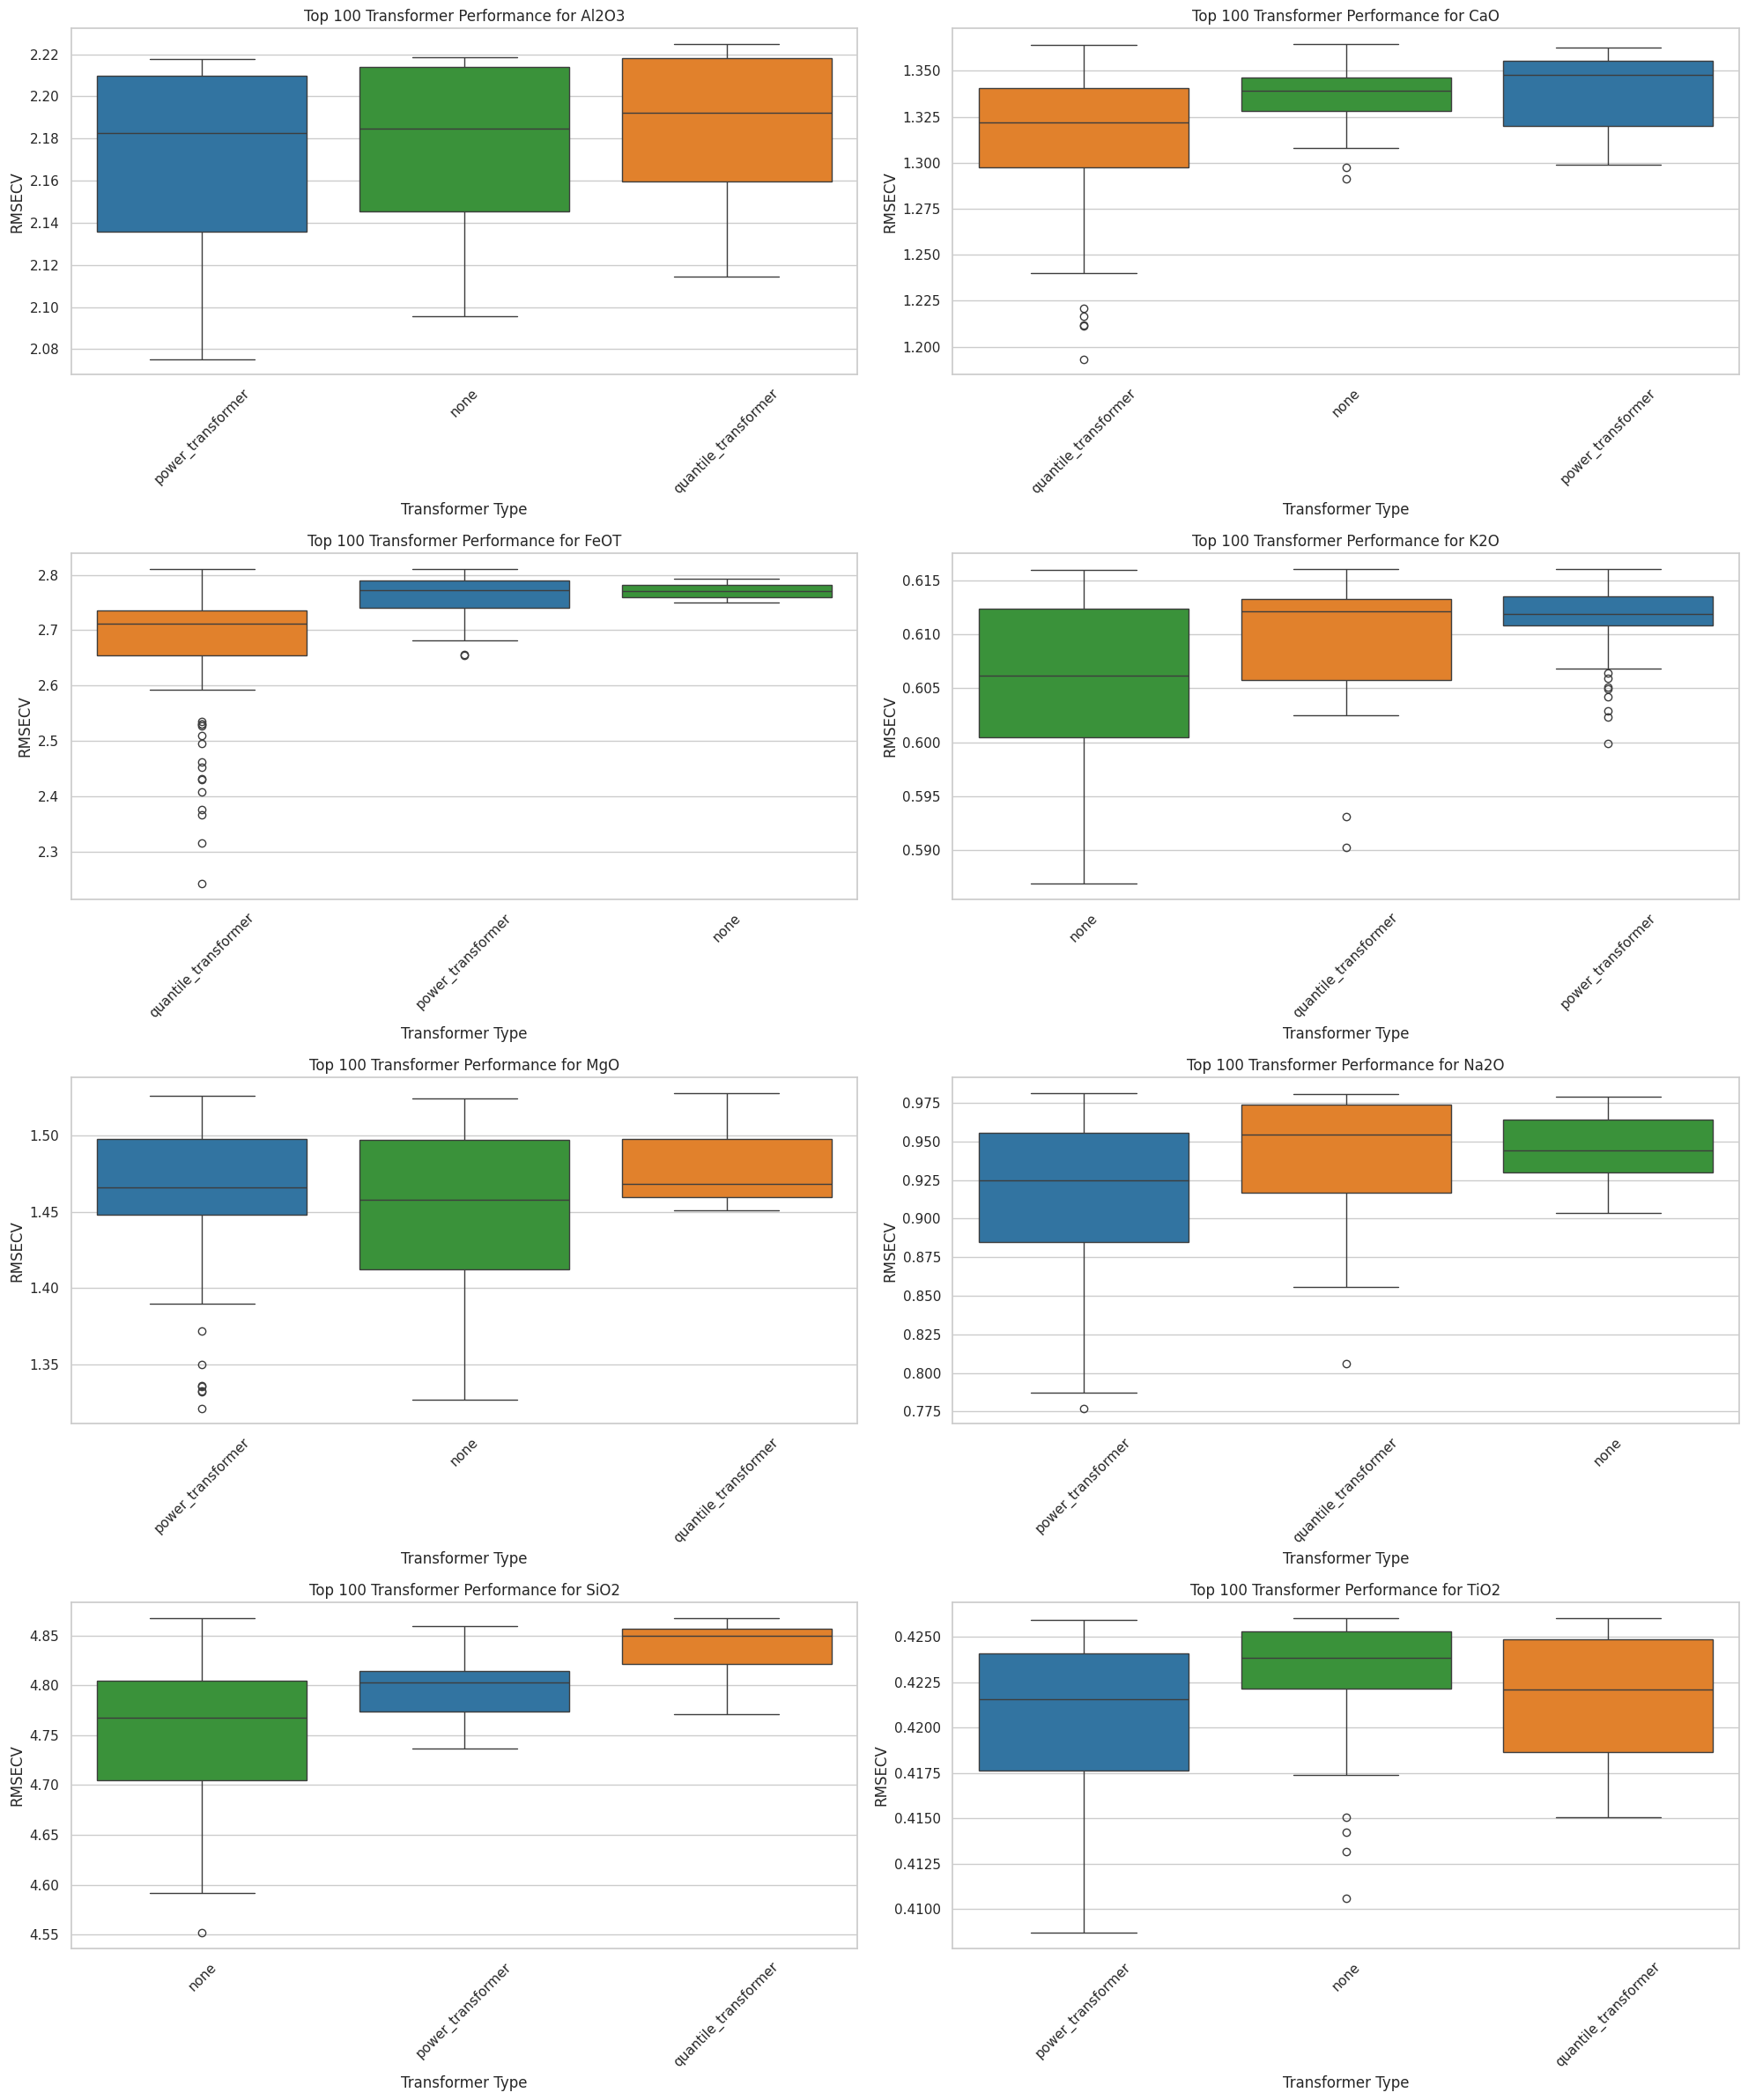
\includegraphics[width=\textwidth]{images/top100/transformers.png}
    \caption{Top 100 transformer performance across oxides. The subplots display the distribution of \gls{rmsecv} values for the top 100 trials for each transformer type across the different oxides. This helps determine the effectiveness of each transformer for different oxides within the top-performing trials.}
    \label{fig:top100_transformers}
\end{figure*}

\begin{figure*}
    \centering
    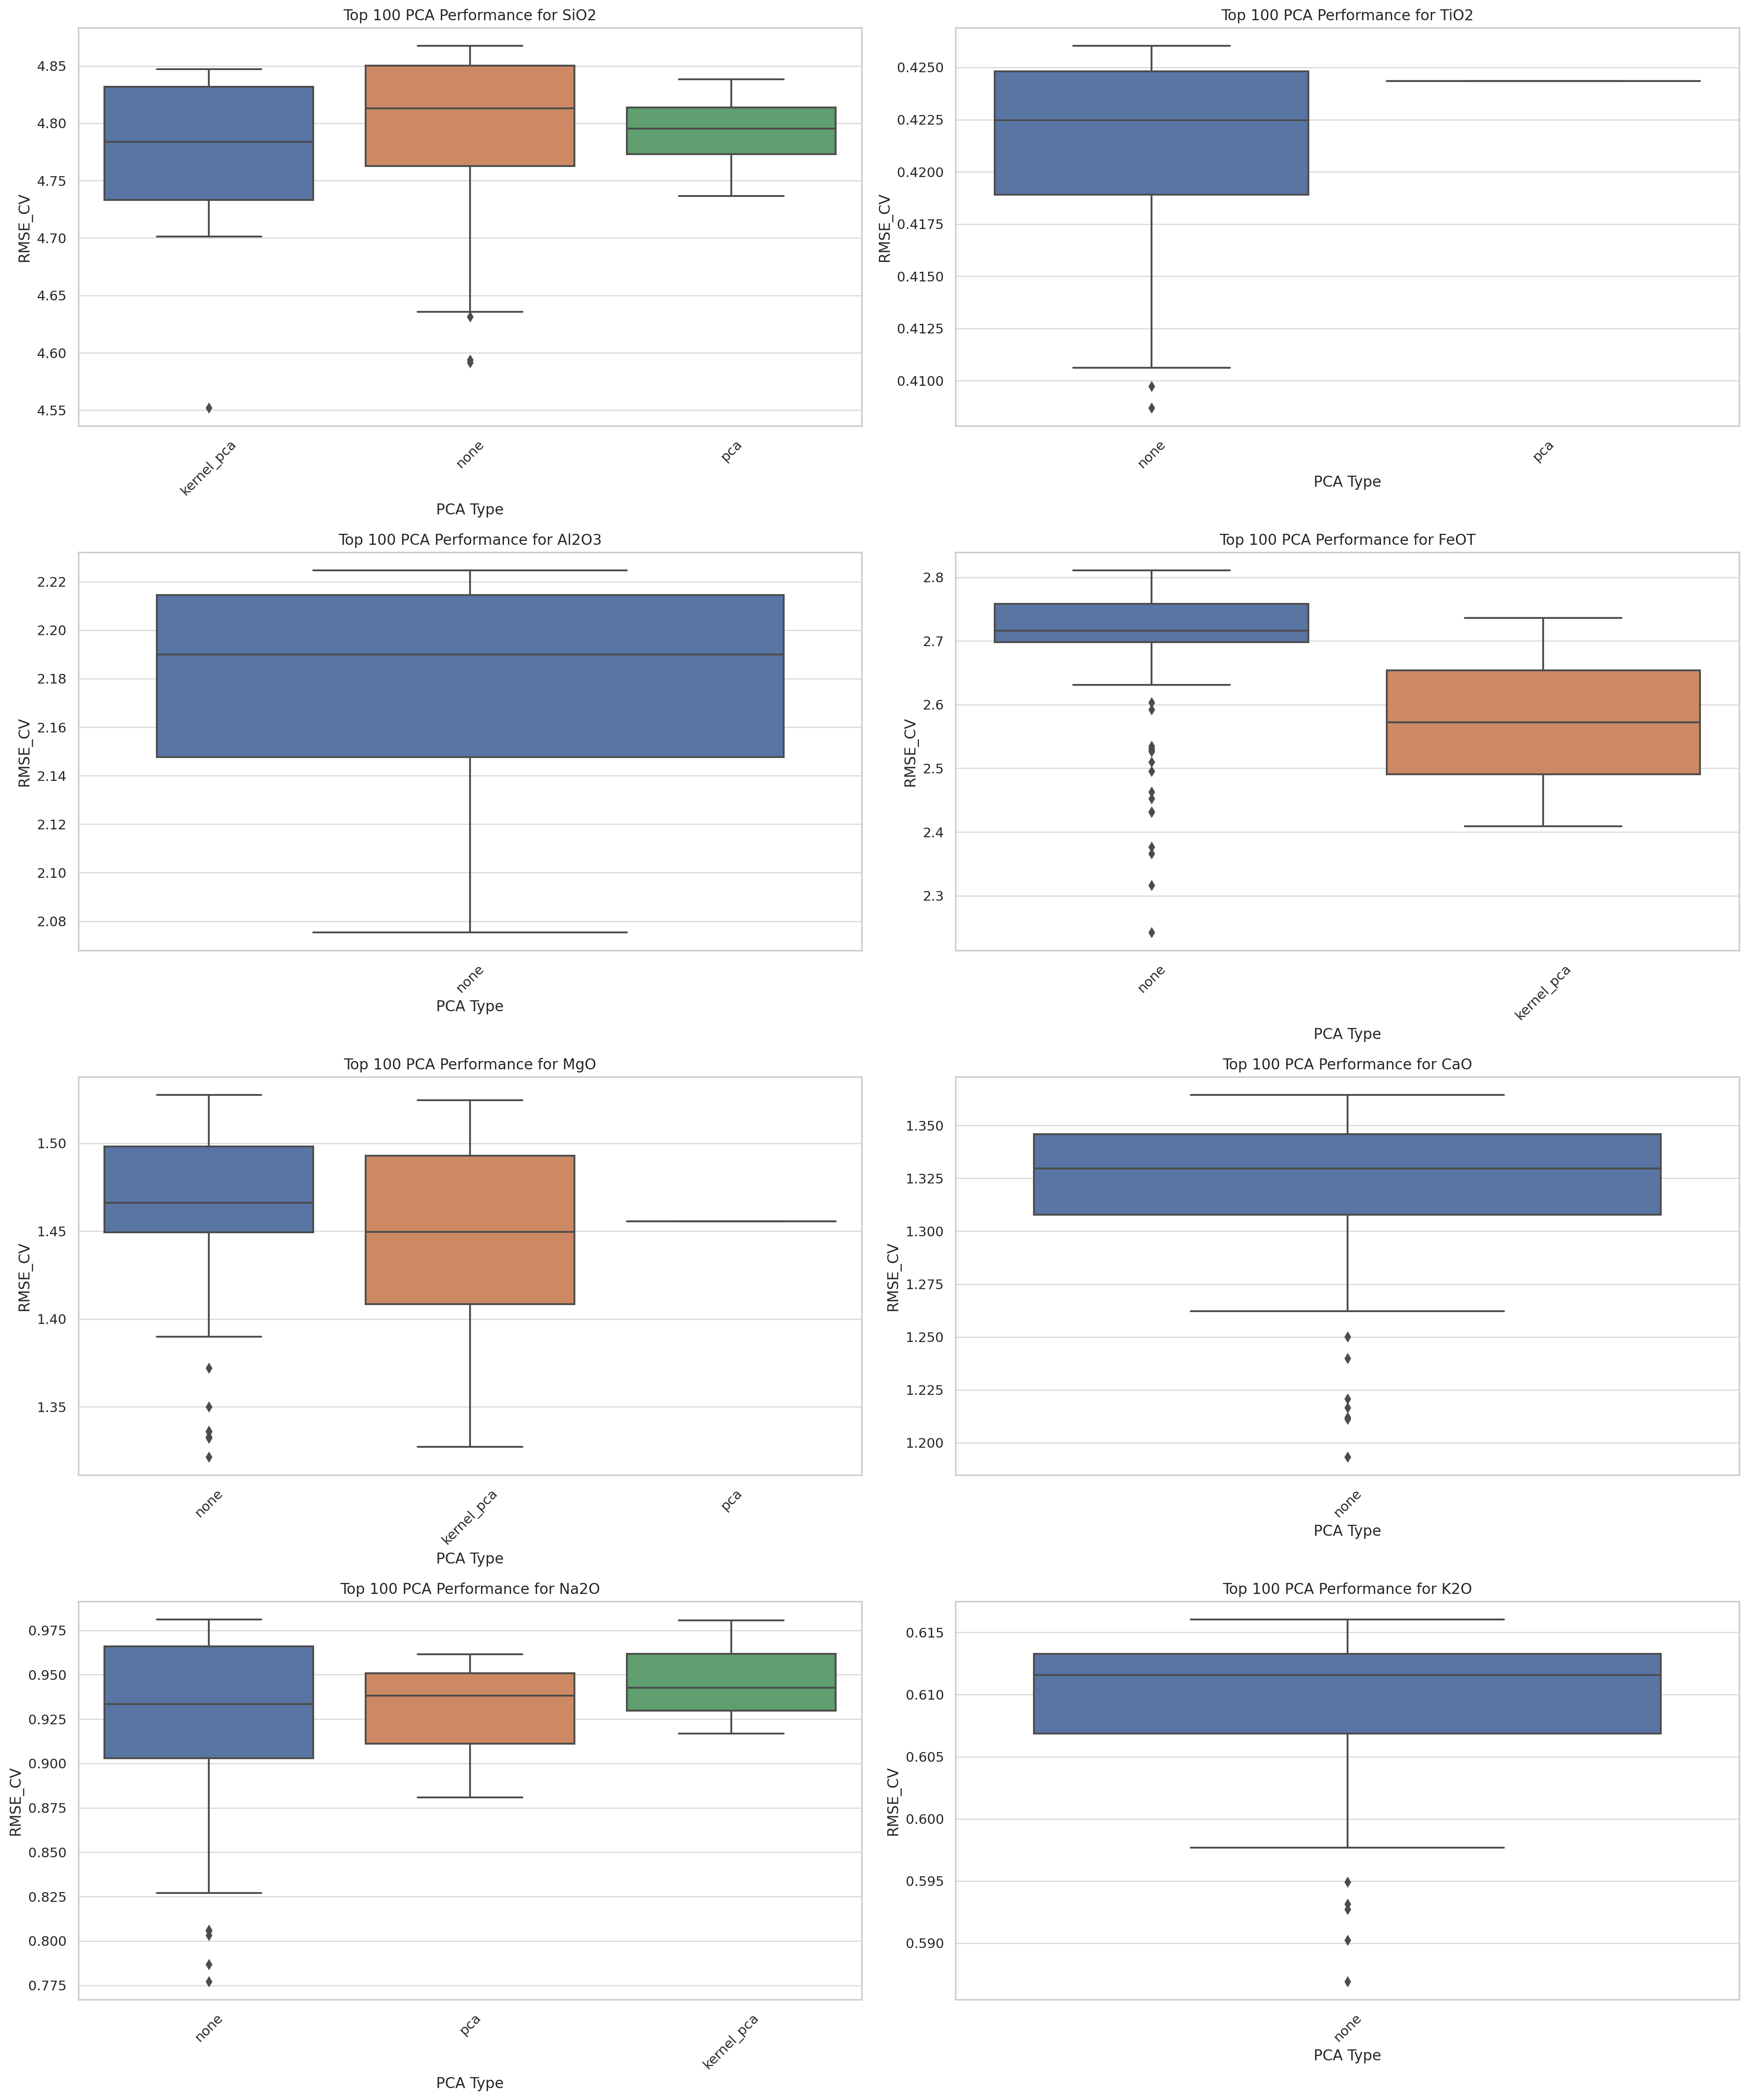
\includegraphics[width=\textwidth]{images/top100/pca.png}
    \caption{Top 100 \gls{pca} performance across oxides. The subplots present the distribution of \gls{rmsecv} values for the top 100 trials for each \gls{pca} type across the different oxides. This allows us to understand the impact of \gls{pca} techniques on model performance for each oxide within the top-performing trials.}
    \label{fig:top100_pca}
\end{figure*}

We conclude our analysis by presenting the best configurations for each oxide in Section~\ref{subsec:best_model_configurations}.
The section shows the single top-performing configurations for each model for each oxide, presented in Tables~\ref{tab:SiO2_best_configurations} through~\ref{tab:K2O_best_configurations}.
Similar to the previous plots, we use the \gls{rmsecv} values to determine the best configurations.
Notably, these tables illustrate how certain configurations may exhibit low \gls{rmsecv} values but relatively high \gls{rmsep} values.
This observation could suggest that they generalize well to the dataset containing extreme values but struggle with values closer to the mean.
For example, the top-performing configuration for \ce{SiO2} consists of \gls{pls} with \gls{kernel-pca} and \texttt{MinMaxScaler}.
This configuration has the lowest \gls{rmsecv} value of 4.55, but a relatively high \gls{rmsep} value of 4.08.
The next-best performing configuration for \ce{SiO2} is \gls{svr} with \texttt{MinMaxScaler}.
This configuration has a \gls{rmsecv} value of 4.59, but a \gls{rmsep} value of 3.53.
Although the difference in \gls{rmsecv} is negligible, the \gls{rmsep} value for the \gls{svr} configuration is much lower than that of the \gls{pls} configuration.
This indicates that the \gls{svr} configuration is likely a better overall predictor for \ce{SiO2} than the \gls{pls} configuration.

The analysis of the best configurations for each oxide reveals that certain models and preprocessing techniques consistently outperform others. \gls{svr} and \gls{pls} models, in particular, frequently appear among the top configurations. The use of transformers such as the Power Transformer and scalers like Norm 3 and Min-Max Scaler are also common among the best configurations.

Finally, we use a combination of these top-performing configurations by selecting the top-$n$ performing configurations per oxide for our stacking ensemble.
This approach is further elaborated on in Section~\ref{subsec:stacking_ensemble}.